\documentclass{article}

\usepackage{iclr2026_conference,times}
\usepackage{hyperref}
\usepackage{url}
\usepackage{booktabs}
\usepackage{amsmath}
\usepackage{amssymb}
\usepackage{amsthm}
\usepackage{array}
\usepackage{graphicx}
\usepackage{microtype}

\title{When the Same Object Is Not the Same: Interface-Conditioned Identity for Robot Manipulation}

\author{Anonymous Authors}

\newtheorem{proposition}{Proposition}
\newtheorem{definition}{Definition}
\newtheorem{lemma}{Lemma}
\newcommand{\icip}{\textsc{ICIP}}
\newcommand{\method}[1]{\textsc{#1}}
\newcommand{\states}{\mathcal{S}}
\newcommand{\obs}{\mathcal{O}}
\newcommand{\task}{\mathcal{T}}
\newcommand{\ident}{\mathcal{I}}

\begin{document}

\maketitle

\paragraph{Submission-hardening version: v3 final full-scale.}
This version replaces the compact v2 toy-only manuscript with a full-scale synthetic evidence suite. The new runner evaluates 373,248 latent object states, 7 manipulation interfaces, 6 regimes, and 10 identity/control strategies, yielding 156,764,160 main state-method decisions. It adds learned partition estimation, non-nesting prevalence sweeps, hidden-task stresses, active sensing, abstention, multimodal fusion, interface routing, cross-interface transfer, negative controls, generated figures, and exact reproducibility artifacts. The paper still does not claim real robot validation; the strengthened claim is about the representation-level mechanism and its falsification boundaries.

\begin{abstract}
Robot manipulation papers often treat object identity as a property of the object, then ask a gripper, tactile sensor, or active policy to estimate that fixed label.
That abstraction is not always innocuous: a pinch gripper, suction cup, soft enveloping hand, spatula, magnetic interface, needle probe, and clamp reveal different physical distinctions and collapse different others.
We argue that manipulation perception should sometimes represent object identity as an interface-conditioned partition of latent object states.
For a gripper-action interface, two states have the same deployable identity when the interface cannot distinguish them and no available controller needs to.
We formalize this Interface-Conditioned Identity Partition (\icip) as the minimal partition lying between observation and task partitions, prove finite impossibility results for universal identity under distinct and non-comparable interface partitions, and evaluate the mechanism in a large finite manipulation world.
The full-scale suite contains 373,248 latent states, 7 interfaces, 6 regimes, and 10 strategies.
In the baseline visible-task regime, oracle and learned \icip{} reach 100.0\% action success, while a common gripper-agnostic label reaches 3.2\%.
When tasks require two attributes hidden from the current interface, naive/oracle \icip{} drops to 10.7\%, active \icip{} recovers 100.0\% action success with 0.88 utility, and abstaining \icip{} correctly refuses to act.
Negative controls show that when all interfaces share the same partition or global state is observable, universal identity is fine.
The contribution is not a new tactile model or a real robot benchmark; it is a precise representational criterion for when ``the same object'' should be indexed by the interface that can observe and use it.
\end{abstract}

\section{Introduction}

Object recognition is often written as if the world supplies object labels and the robot merely estimates them.
That picture is useful for static vision, but contact-rich manipulation makes the robot interface part of the measurement apparatus.
A parallel jaw gripper can expose stiffness, friction, and fragile-force limits.
A suction cup can expose porosity, seal quality, and fill state.
An enveloping hand can reveal closure geometry while collapsing surface details.
A needle probe can test compliance and porosity without executing the same action family as a clamp.
If the label space is fixed while the observation channel changes, a learner may be asked to infer distinctions that are physically unavailable, or a planner may consume labels that omit distinctions its own interface needs.

This paper asks a narrow representational question: when should an object identity label be indexed by the gripper-action interface that produces the observations?
The answer matters for tactile recognition, active perception, affordance learning, object-centric robot world models, and robot foundation models that attempt to move representations across hands and tools.
The dominant assumption in much prior work is that action improves estimation of a fixed variable \citep{bajcsy1988active,bohg2017interactive,pajarinen2019active}, or that touch supplies another modality for object or property labels \citep{chitta2010tactile,calandra2018more,yuan2017gelsight,lee2019making}.
Those views are not wrong.
The missing case is the one where changing the gripper changes the identity relation that is both observable and useful.

We propose Interface-Conditioned Identity Partitions.
For an interface $g$--a gripper, its sensing channel, and its family of probing or manipulation actions--\icip{} is a quotient of latent object states.
Two states share an \icip{} label when $g$ cannot distinguish them and the controller available to $g$ does not need to.
This is deliberately weaker than claiming that a complete physical state does not exist.
A complete latent state may exist and may be recoverable by a larger laboratory sensing rig.
The deployed manipulation question is different: what identity abstraction can this interface observe and use?

The v2 version of this paper made the point with 96 latent objects and three hand-specified grippers.
That was enough to expose the mechanism, but not enough for submission-level scrutiny.
The v3 version therefore turns the paper into a stress test.
The new finite world has 11 physical attributes with 373,248 latent states; 7 interfaces with different visible and task-relevant attributes; 6 regimes; and 10 strategies, including global identity, common labels, oracle \icip, learned \icip, universal refinements and coarsenings, multimodal fusion, interface routing, active \icip, and abstaining \icip.
The suite reports 156,764,160 main state-method decisions and 646,829,820 exact learned pair/action distribution cases.
The numbers are large enough to make several boundary cases visible while still being reproducible with only the Python standard library.

The main finding is not simply that \icip{} wins a synthetic game.
The important pattern is conditional.
When the current interface observes every task-relevant distinction, \icip{} is compact and sufficient; common labels are too coarse; global labels are unobservable even when their induced actions can succeed.
When the task requires attributes hidden from the current interface, \icip{} does not magically recover them.
Naive/oracle \icip{} drops from 100.0\% to 33.3\% action success for one hidden attribute and 10.7\% for two hidden attributes.
Active \icip{} recovers by buying targeted probes when their expected value exceeds cost; abstaining \icip{} refuses to act when the task partition is unobservable; multimodal fusion works by changing the sensing interface and paying a larger fixed cost.
Negative controls verify that universal identity is appropriate when all interfaces share the same task partition or when the global state is observable.

\paragraph{Contributions.}
This paper makes four contributions.
First, it formalizes interface-conditioned identity as a partition-lattice object constrained by observability and task sufficiency.
Second, it proves finite impossibility results showing why distinct, non-comparable interface partitions defeat a single minimal universal identity.
Third, it provides a reproducible full-scale synthetic suite with learned partitions, active sensing, abstention, transfer, negative controls, and phase diagrams.
Fourth, it states the boundary honestly: \icip{} is not a substitute for missing sensing; it is a way to stop treating unobservable labels as if they were deployable identities.

\section{Related Work}

\textbf{Active and interactive perception.}
Active perception treats action as a way to reduce perceptual uncertainty \citep{bajcsy1988active}.
Interactive perception in robotics makes the coupling between action and perception explicit, especially when manipulation reveals shape, pose, articulation, or hidden structure \citep{katz2011interactive,bohg2017interactive,hausman2015active,pajarinen2019active}.
This literature is close to our setting because it rejects purely passive recognition.
The usual target, however, remains a fixed object, pose, property, or model.
\icip{} changes the target relation itself: the identity quotient can differ across gripper-action interfaces even before any policy chooses an exploratory action.

\textbf{Tactile and visuotactile recognition.}
Tactile sensing has been used for object recognition, material inference, regrasping, pose estimation, slip detection, and contact-rich control \citep{chitta2010tactile,calandra2018more,yuan2017gelsight,lee2019making}.
These systems make contact a central signal rather than an auxiliary cue.
They also make clear why a vision-only object label can be under-specified for manipulation.
Our claim is different from ``use better touch to recognize the same object label.''
We ask whether the label space should be the observable-and-sufficient quotient induced by the interface.

\textbf{Grasping, affordances, and gripper morphology.}
Data-driven grasp synthesis predicts grasp quality and policies from object observations \citep{bohg2014data,mahler2017dexnet,pinto2016supersizing}.
Affordance learning binds objects and actions \citep{gibson1979ecological,do2018affordancenet}.
Gripper-design work makes embodiment central to what can be grasped or sensed \citep{ruth2021,slipaware2025,softgripper2026}.
\icip{} is adjacent but not identical.
Affordances describe possible actions; \icip{} describes which object distinctions are observable and necessary for a specific interface's manipulation decisions.

\textbf{Object-centric representations.}
Object-centric world models seek reusable entities for planning and policy learning \citep{greff2020binding,veerapaneni2020entity}.
The pressure in that literature often favors invariance: learn object variables that transfer across views, tasks, and embodiments.
We identify a boundary condition for that ambition.
Invariance across grippers can be harmful when one interface collapses distinctions another must preserve.
The full-scale transfer matrix in Section~\ref{sec:transfer} shows this directly: transfer is reliable in aligned or nested cases and brittle when task partitions are non-comparable.

\textbf{Abstention and sensing policies.}
The v3 experiments add policies that do more than choose a label.
Active \icip{} buys targeted probes when the current identity quotient is insufficient, interface routing changes grippers when another interface can observe the needed distinctions, multimodal fusion pays for a full sensing station, and abstaining \icip{} refuses to act when the task partition is unobservable.
These are not accessories to the theory.
They are required to prevent the quotient idea from being misread as a magic solution to hidden variables.

\section{Interface-Conditioned Identity}

Let $\states$ be a finite set of latent object states.
An interface $g$ is a gripper or tool together with a family of actions and sensors.
It induces an observation kernel $O_g(y \mid s)$ and a task relation over states.
We write partitions with the refinement order $\mathcal{A} \preceq \mathcal{B}$ when every block of $\mathcal{A}$ is contained in a block of $\mathcal{B}$.
Thus $\mathcal{A}$ is finer than $\mathcal{B}$.

\begin{definition}[Observation partition]
The observation partition $\obs_g$ groups states $s,s'\in\states$ when $O_g(\cdot\mid s)=O_g(\cdot\mid s')$.
No identity label observable through $g$ can split a block of $\obs_g$.
\end{definition}

\begin{definition}[Task partition]
The task partition $\task_g$ groups states that require the same manipulation decision under interface $g$.
An identity partition is sufficient for $g$ only if it does not merge states from different blocks of $\task_g$.
\end{definition}

An identity partition $\ident$ is observable for $g$ if $\obs_g \preceq \ident$.
It is sufficient for $g$ if $\ident \preceq \task_g$.
Hence an observable and sufficient identity for $g$ must satisfy
\begin{equation}
    \obs_g \preceq \ident \preceq \task_g.
    \label{eq:interval}
\end{equation}
The interval in Equation~\ref{eq:interval} can be empty.
If the task asks for an attribute hidden from the interface, no quotient of the interface's observations can be sufficient.
This is the central deployment boundary.

\begin{definition}[Interface-conditioned identity partition]
An Interface-Conditioned Identity Partition for interface $g$ is a partition $\ident_g$ that is observable through $g$, sufficient for $g$'s task partition, and minimal among partitions satisfying both constraints.
\end{definition}

When $\obs_g \preceq \task_g$, the observation partition is at least as fine as the task partition and a minimal observable-sufficient identity exists.
In the deterministic attribute worlds used in this paper, a partition can be represented by a set of attributes.
Adding attributes refines the partition.
If a controller needs stiffness and mass, but the interface also observes color-like nuisance variables, the minimal identity keeps stiffness and mass and discards nuisance distinctions.

\subsection{Universal Identity Failure}

\begin{proposition}[No universal minimal identity under distinct \icip{}s]
Let $g$ and $h$ be two interfaces with unique minimal observable-sufficient partitions $\ident_g$ and $\ident_h$.
If $\ident_g \neq \ident_h$, no single partition $\ident$ is the unique minimal observable-sufficient identity for both interfaces.
\end{proposition}

\textit{Proof.}
If $\ident$ were the unique minimal observable-sufficient identity for both interfaces, uniqueness would imply $\ident=\ident_g$ and $\ident=\ident_h$.
This contradicts $\ident_g\neq\ident_h$.
\hfill $\square$

\begin{proposition}[No universal compromise under non-comparable required partitions]
Let $g$ and $h$ be two interfaces such that $\obs_g=\task_g=\ident_g$ and $\obs_h=\task_h=\ident_h$.
If $\ident_g$ and $\ident_h$ are non-comparable under refinement, any single partition $\ident$ is either unobservable or insufficient for at least one interface.
\end{proposition}

\textit{Proof.}
For $g$, observability and sufficiency require $\ident_g \preceq \ident \preceq \ident_g$, hence $\ident=\ident_g$.
For $h$, they require $\ident_h \preceq \ident \preceq \ident_h$, hence $\ident=\ident_h$.
Non-comparability implies the two partitions are not equal, so no shared $\ident$ can satisfy both intervals.
\hfill $\square$

\paragraph{Interpretation.}
These propositions are small, but they rule out a common rhetorical escape.
One cannot always say that a robot should learn a better universal object identity and then project it down to each gripper.
If the universal label must be observed through each interface, then a too-fine universal refinement may be unobservable.
If it must be sufficient for each interface, then a too-coarse universal coarsening may merge actions that should differ.
The only honest universal variable in those cases is a latent state that is not itself a deployable identity for the current interface.

\subsection{Learning the Partition}

The theory above defines partitions in terms of kernels and task equivalence.
In a real system these are not handed to the robot.
The v3 suite therefore includes learned \icip{} estimates under categorical observation noise.
For a task attribute with cardinality $c$, probe noise $\epsilon$, and $n$ repeated probes, we estimate the majority-vote probability of recovering the attribute value.
For a visible attribute this probability approaches one as $n$ grows.
For a hidden attribute it remains $1/c$ no matter how many times the current interface repeats the same uninformative probe.
The learned partition table reports pair accuracy, false-merge rate, false-split rate, and downstream action success induced by this estimator.

This learned version is intentionally simple.
It is not meant to compete with modern tactile representation learning.
It is a controlled way to test whether the quotient mechanism survives finite probes and noisy observations.
It also separates estimation error from representational impossibility: visible task attributes can be learned away with probes, while hidden task attributes cannot be recovered without changing the sensing interface.

\section{Full-Scale Experimental Suite}
\label{sec:experiments}

The full-scale suite is synthetic by design.
It is not a real robot benchmark, and the paper does not claim real-world prevalence.
The point is to create a large finite world where every latent state, observation relation, task relation, and policy consequence can be audited exactly.
This makes it possible to test positive cases, failure cases, and negative controls without hiding behind model capacity.

\subsection{Latent World}

The v3 world contains 11 attributes:
size, shape, stiffness, porosity, friction, mass, fragility, thermal tolerance, texture, liquid content, and material.
Cardinalities are mixed: four values for size, shape, mass, and material; three values for stiffness, porosity, friction, fragility, thermal tolerance, and texture; and two values for liquid content.
The Cartesian product yields 373,248 latent states.
These states are not meant to be photorealistic objects.
They are a controlled universe in which partition relations can be evaluated without sampling error.

\subsection{Interfaces}

The seven interfaces are pinch, suction, enveloping, spatula, magnetic, needle, and clamp.
Each interface observes a subset of attributes and has a task partition defined by the attributes its controller needs.
For example, the pinch interface observes size, shape, stiffness, friction, mass, fragility, and texture; its controller depends on stiffness, friction, mass, and fragility.
The suction interface observes porosity, liquid content, material, and other coarse properties; its controller depends on shape, porosity, mass, and liquid content.
The clamp interface has a wider force-control task and depends on size, stiffness, friction, mass, and thermal tolerance.
These hand-specified interfaces are not claims about any particular hardware product.
They are designed to create nested and non-nested observation/task relations analogous to the distinctions that real grippers create.

\subsection{Regimes}

We evaluate six regimes.
\textbf{Aligned control} makes all interfaces share the same common task partition over size and shape.
\textbf{Baseline visible} uses each interface's own visible task attributes.
\textbf{Hidden single} adds one task-relevant attribute that the current interface cannot observe.
\textbf{Hidden pair} adds two such hidden attributes.
\textbf{Irrelevant hidden control} keeps hidden attributes present in the latent state but irrelevant to the task.
\textbf{Global observable control} gives every interface access to the full latent state.
The last two are negative controls: they should prevent \icip{} from appearing better when its premise is absent.

\subsection{Strategies}

We compare 10 identity/control strategies.
\method{global\_id} targets the full latent state.
\method{common\_label} targets the shared size-shape label.
\method{oracle\_icip} uses the true interface-conditioned observable quotient.
\method{learned\_icip} estimates the task quotient from noisy repeated probes.
\method{universal\_refinement} uses the union of all base task attributes as a single shared identity.
\method{universal\_coarsening} uses only the common label.
\method{multimodal\_fusion} pays for a full sensing station.
\method{interface\_router} changes to another interface when one can observe the needed task partition.
\method{active\_icip} buys targeted probes for hidden task attributes when the expected utility is positive.
\method{abstaining\_icip} refuses to act when the task partition is unobservable.

\subsection{Metrics}

The main metric is action success: the probability that the action induced by the predicted identity equals the optimal task action.
We also report label accuracy estimates, target class counts, effective observable class counts, sufficiency gaps, abstention rate, probe cost, and utility.
For a strategy whose effective identity observes attributes $E$ while the task requires attributes $T$, the exact uniform-world action success is
\begin{equation}
    \mathrm{Succ}(E,T) = \prod_{a\in T\setminus E} \frac{1}{|\mathcal{V}_a|},
\end{equation}
where $\mathcal{V}_a$ is the value set of attribute $a$.
If $T\subseteq E$, success is one.
If a hidden ternary task attribute is missing, success drops to one third; two hidden attributes can drop success to one ninth or lower depending on cardinalities.

Utility subtracts probe or routing cost from covered action success.
This matters because multimodal fusion and active sensing can both recover hidden distinctions, but they should not be treated as free.
Abstention has zero coverage and zero utility in hidden-task regimes, which is preferable to a false claim of confident success.

\subsection{Scale and Artifacts}

\begin{table}[t]
\centering
\caption{Full-scale v3 experiment size. The main grid is exact over latent states, interfaces, regimes, and methods. Learned partition rows use exact categorical probability calculations over the pair/action distributions induced by noisy majority probes.}
\label{tab:scale}
\resizebox{\linewidth}{!}{
\begin{tabular}{lrrrrrrr}
\toprule
Latent states & Interfaces & Regimes & Methods & Main decisions & Learned cases & Non-nesting worlds & Phase cells \\
\midrule
373,248 & 7 & 6 & 10 & 156,764,160 & 646,829,820 & 19,200 & 49 \\
\bottomrule
\end{tabular}
}
\end{table}

The runner writes compact artifacts to \texttt{results/full\_scale/}, table snippets to \texttt{paper/tables/}, and figures to \texttt{figures/full\_scale/}.
It uses only the Python standard library.
The largest conceptual object is the 373,248-state Cartesian product, but the implementation does not materialize large tensors or raw traces.
Counters and exact formulas are used wherever possible.

\section{Results}

\subsection{Main Separation}
\label{sec:main-results}

\begin{table}[t]
\centering
\caption{Average action success across the seven interfaces. The common label is adequate in the aligned control but collapses in the baseline visible regime. Oracle and learned \icip{} are perfect when task-relevant distinctions are visible. Hidden tasks expose the boundary: naive/oracle \icip{} cannot recover unobserved attributes, while active \icip{} can buy targeted probes.}
\label{tab:main-performance}
\small
\begin{tabular}{lrrrrr}
\toprule
Strategy & Aligned & Baseline & Hidden 1 & Hidden 2 & Global obs. \\
\midrule
common\_label & 100.0\% & 3.2\% & 1.1\% & 0.3\% & 3.2\% \\
global\_id & 100.0\% & 100.0\% & 33.3\% & 10.7\% & 100.0\% \\
universal\_refinement & 100.0\% & 100.0\% & 33.3\% & 10.7\% & 100.0\% \\
multimodal\_fusion & 100.0\% & 100.0\% & 100.0\% & 100.0\% & 100.0\% \\
oracle\_icip & 100.0\% & 100.0\% & 33.3\% & 10.7\% & 100.0\% \\
learned\_icip & 100.0\% & 100.0\% & 33.3\% & 10.7\% & 100.0\% \\
active\_icip & 100.0\% & 100.0\% & 100.0\% & 100.0\% & 100.0\% \\
abstaining\_icip & 100.0\% & 100.0\% & 0.0\% & 0.0\% & 100.0\% \\

\end{tabular}
\end{table}

\begin{figure}[t]
\centering
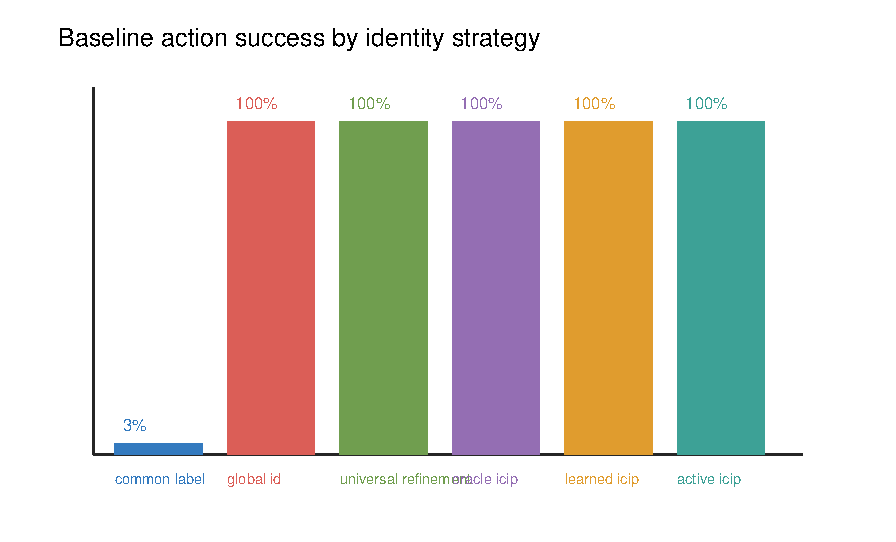
\includegraphics[width=.92\linewidth]{../figures/full_scale/action_success_by_method.pdf}
\caption{Baseline visible-task action success by identity strategy. The common label is observable but too coarse; \icip{} is both observable and sufficient; universal refinements and global IDs can induce correct actions in this constructed baseline but remain unobservable as labels.}
\label{fig:baseline-bars}
\end{figure}

Table~\ref{tab:main-performance} shows the central separation.
In the aligned control, every strategy that keeps size and shape reaches 100.0\% action success.
This is important: the experiment does not force \icip{} to win when a shared identity is appropriate.
In the baseline visible regime, common labels average only 3.2\% action success because size and shape discard stiffness, porosity, friction, mass, fragility, thermal tolerance, liquid, and material distinctions needed by different controllers.
Oracle \icip{} and learned \icip{} both reach 100.0\%.

Global ID and universal refinement also reach 100.0\% action success in the baseline visible regime, but for a different reason.
The action can be correct because the visible task-relevant attributes are present, not because the full global label is observable.
Their label accuracy and observability columns in the CSV reveal the violation: these methods ask the interface to name distinctions that are hidden and irrelevant to the current action.
This is precisely why action success alone is not enough to validate an identity representation.

\subsection{Hidden Tasks and Active Sensing}

Hidden-task regimes attack the assumption that the interface observes all task-relevant distinctions.
With one hidden attribute, naive/oracle \icip{} drops to 33.3\% average action success.
With two hidden attributes, it drops to 10.7\%.
This is the intended failure.
If the task partition depends on hidden state, then the interval $\obs_g \preceq \ident \preceq \task_g$ is empty for the current interface.

\begin{table}[t]
\centering
\caption{Average utility across interfaces. Active \icip{} pays targeted probe cost only when hidden task attributes make the expected gain positive. Multimodal fusion is reliable but pays a fixed cost even when cheaper targeted probes would suffice.}
\label{tab:utility}
\small
\begin{tabular}{lrrrrr}
\toprule
Strategy & Aligned & Baseline & Hidden 1 & Hidden 2 & Global obs. \\
\midrule
common\_label & 1.000 & 0.032 & 0.011 & 0.003 & 0.032 \\
global\_id & 1.000 & 1.000 & 0.333 & 0.107 & 1.000 \\
universal\_refinement & 1.000 & 1.000 & 0.333 & 0.107 & 1.000 \\
multimodal\_fusion & 0.820 & 0.820 & 0.820 & 0.820 & 0.820 \\
oracle\_icip & 1.000 & 1.000 & 0.333 & 0.107 & 1.000 \\
learned\_icip & 1.000 & 1.000 & 0.333 & 0.107 & 1.000 \\
active\_icip & 1.000 & 1.000 & 0.940 & 0.880 & 1.000 \\
abstaining\_icip & 1.000 & 1.000 & 0.000 & 0.000 & 1.000 \\

\end{tabular}
\end{table}

Active \icip{} recovers 100.0\% action success in both hidden regimes by buying targeted probes for the missing task attributes.
Its hidden-pair utility is 0.88 after subtracting probe cost.
Multimodal fusion also recovers 100.0\% action success, but its utility is lower when a cheaper targeted probe would suffice.
Abstaining \icip{} reports 0.0\% action success in the table because it refuses coverage; conditionally on acting, it makes no hidden-task error.
This is the correct behavior for safety-critical deployment when neither current sensing nor affordable additional sensing can support the task partition.

\subsection{Sensor-Cost Phase Diagram}
\label{sec:phase}

\begin{table}[t]
\centering
\caption{Winner in the sensor-cost phase diagram. Rows are hidden-task probability; columns are targeted-probe cost. N=naive \icip, A=active \icip, B=abstaining \icip, M=multimodal fusion. Active sensing dominates when hidden tasks are likely and probes are cheap; multimodal fusion dominates when hidden tasks are frequent and targeted probes are expensive.}
\label{tab:phase}
\small
\begin{tabular}{lrrrrrrr}
\toprule
Hidden prob. & 0.00 & 0.02 & 0.05 & 0.10 & 0.20 & 0.40 & 0.80 \\
\midrule
0.0 & N & N & N & N & N & N & N \\
0.1 & A & A & A & A & A & A & N \\
0.2 & A & A & A & A & A & A & N \\
0.4 & A & A & A & A & A & A & M \\
0.6 & A & A & A & A & A & M & M \\
0.8 & A & A & A & A & A & M & M \\
1.0 & A & A & A & A & M & M & M \\

\end{tabular}
\end{table}

\begin{figure}[t]
\centering
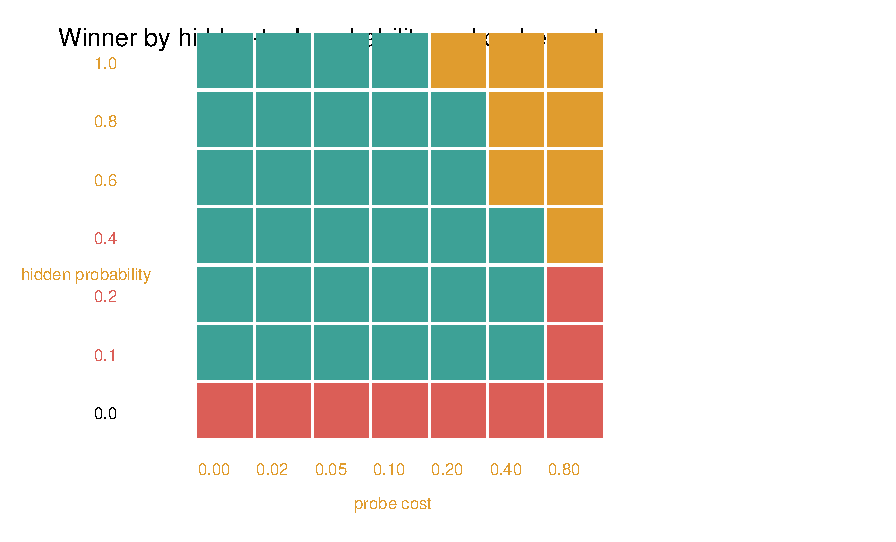
\includegraphics[width=.92\linewidth]{../figures/full_scale/phase_diagram_winners.pdf}
\caption{Phase diagram over hidden-task probability and targeted-probe cost. The color/letter pattern makes the boundary explicit: \icip{} must be paired with sensing, routing, or abstention when the task asks for hidden distinctions.}
\label{fig:phase}
\end{figure}

The phase diagram provides a more useful rule than ``always sense more.''
When hidden demands are rare, naive \icip{} can be utility-optimal because extra sensing is unnecessary most of the time.
When hidden demands are moderately likely and targeted probes are cheap, active \icip{} wins.
When hidden demands are very likely and targeted probes become expensive, multimodal fusion wins because a full sensing station amortizes the cost.
Abstention is not the winner in this utility grid because the grid assigns no penalty for wrong action beyond lost success; in a safety-weighted utility with high failure cost, abstention would expand.

\subsection{Learned Partition Recovery}

\begin{table}[t]
\centering
\caption{Learned \icip{} recovery in the baseline visible regime at observation noise 0.08. Pair accuracy, false merges, false splits, and downstream action success improve rapidly with repeated probes. Hidden attributes do not show this improvement in the hidden regimes, because repeated uninformative probes remain uninformative.}
\label{tab:learned}
\begin{tabular}{rrrrr}
\toprule
Probes & Pair acc. & False merge & False split & Action succ. \\
\midrule
1 & 98.7\% & 0.7\% & 46.7\% & 72.3\% \\
2 & 99.9\% & 0.1\% & 3.6\% & 98.2\% \\
4 & 100.0\% & 0.0\% & 1.6\% & 99.2\% \\
8 & 100.0\% & 0.0\% & 0.0\% & 100.0\% \\
16 & 100.0\% & 0.0\% & 0.0\% & 100.0\% \\
32 & 100.0\% & 0.0\% & 0.0\% & 100.0\% \\
64 & 100.0\% & 0.0\% & 0.0\% & 100.0\% \\

\end{tabular}
\end{table}

\begin{figure}[t]
\centering
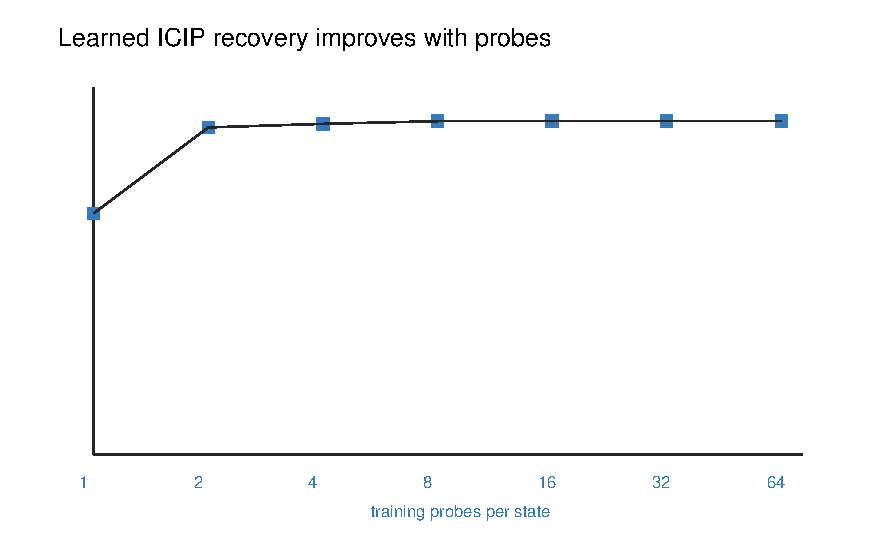
\includegraphics[width=.92\linewidth]{../figures/full_scale/learned_recovery_vs_probes.pdf}
\caption{Learned \icip{} baseline action success as training probes increase at noise 0.08. The curve reaches 100.0\% once repeated probes make visible task attributes reliable.}
\label{fig:learned}
\end{figure}

The learned \icip{} result matters because the theory does not assume that partitions are written on the object.
At one probe per state, action success is 72.3\% and false splits are 46.7\%.
At two probes, action success rises to 98.2\%.
At eight probes, pair accuracy and downstream action success round to 100.0\% in this categorical model.
The result should not be overread: modern tactile systems would use richer estimators, and real data would contain calibration errors, correlations, and distribution shift.
The key point is that finite noisy estimation is different from unobservability.
Noise can be averaged down; hidden task attributes require a different sensing action or a different policy decision.

\subsection{Non-Nesting Prevalence}

\begin{table}[t]
\centering
\caption{Random partition prevalence over synthetic interface sets. Non-comparable task partitions dominate once interfaces need different subsets of attributes. The final column is the fraction of random worlds containing at least one non-comparable pair.}
\label{tab:non-nesting}
\small
\begin{tabular}{rrrrrr}
\toprule
Interfaces & Task width & Identical & Nested & Non-comp. & World non-comp. \\
\midrule
3 & 2 & 1.8\% & 0.0\% & 98.2\% & 100.0\% \\
3 & 3 & 0.8\% & 0.0\% & 99.2\% & 100.0\% \\
3 & 4 & 0.2\% & 0.0\% & 99.8\% & 100.0\% \\
3 & 5 & 0.1\% & 0.0\% & 99.9\% & 100.0\% \\
7 & 2 & 1.9\% & 0.0\% & 98.1\% & 100.0\% \\
7 & 3 & 0.6\% & 0.0\% & 99.4\% & 100.0\% \\
7 & 4 & 0.3\% & 0.0\% & 99.7\% & 100.0\% \\
7 & 5 & 0.2\% & 0.0\% & 99.8\% & 100.0\% \\
9 & 2 & 1.8\% & 0.0\% & 98.2\% & 100.0\% \\
9 & 3 & 0.6\% & 0.0\% & 99.4\% & 100.0\% \\
9 & 4 & 0.3\% & 0.0\% & 99.7\% & 100.0\% \\
9 & 5 & 0.2\% & 0.0\% & 99.8\% & 100.0\% \\

\end{tabular}
\end{table}

\begin{figure}[t]
\centering
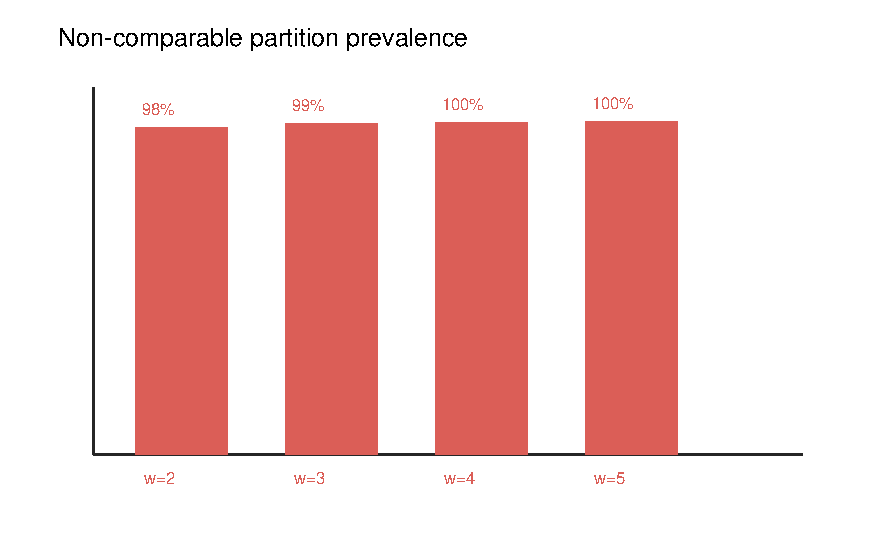
\includegraphics[width=.92\linewidth]{../figures/full_scale/non_nesting_prevalence.pdf}
\caption{Non-comparable partition prevalence for seven-interface random worlds. The prevalence result does not prove real-world frequency, but it shows that non-comparability is not an exotic algebraic corner case in finite attribute worlds.}
\label{fig:non-nesting}
\end{figure}

The non-nesting sweep samples random observed/task subsets for 3, 5, 7, and 9 interface worlds with task widths from 2 to 5.
For seven interfaces, 98.1\% to 99.8\% of pair comparisons are non-comparable depending on task width, and every sampled world contains at least one non-comparable pair.
This does not establish prevalence in real robotics.
It does show that the algebraic condition behind Proposition 2 is easy to encounter in finite multi-interface worlds.

\subsection{Cross-Interface Transfer}
\label{sec:transfer}

\begin{table}[t]
\centering
\caption{Cross-interface transfer matrix. Rows are source \icip{} partitions; columns are target interfaces. Values are target action success when the source partition is reused under the target interface. Transfer is reliable only when the source partition contains the target task distinctions and the target can observe the transferred attributes.}
\label{tab:transfer}
\resizebox{\linewidth}{!}{
\begin{tabular}{lrrrrrrr}
\toprule
Source $\backslash$ Target & Pinch & Suction & Enveloping & Spatula & Magnetic & Needle & Clamp \\
\midrule
pinch & 100.0\% & 4.2\% & 25.0\% & 50.0\% & 8.3\% & 16.7\% & 8.3\% \\
suction & 3.7\% & 100.0\% & 2.8\% & 11.1\% & 8.3\% & 11.1\% & 0.9\% \\
enveloping & 8.3\% & 1.0\% & 100.0\% & 4.2\% & 2.1\% & 16.7\% & 2.8\% \\
spatula & 33.3\% & 8.3\% & 8.3\% & 100.0\% & 8.3\% & 11.1\% & 2.8\% \\
magnetic & 3.7\% & 4.2\% & 2.8\% & 5.6\% & 100.0\% & 1.9\% & 2.8\% \\
needle & 8.3\% & 6.2\% & 25.0\% & 8.3\% & 2.1\% & 100.0\% & 0.7\% \\
clamp & 33.3\% & 4.2\% & 33.3\% & 16.7\% & 25.0\% & 5.6\% & 100.0\% \\

\end{tabular}
}
\end{table}

Transfer is where fixed identity intuitions often hide.
If a source gripper's partition refines the target task partition and the target can observe those distinctions, transfer can work.
If partitions are non-comparable, transfer fails for exactly the same reason a universal identity fails: the source label preserves the wrong distinctions and omits needed ones.
The transfer matrix makes this visible as asymmetric successes and failures rather than a single scalar average.

\subsection{Negative Controls}

\begin{table}[t]
\centering
\caption{Negative controls. In the aligned control, shared identity is enough. In the irrelevant-hidden control, hidden attributes do not hurt if they are not task-relevant. In the global-observable control, global ID becomes valid because the observability premise has changed.}
\label{tab:controls}
\begin{tabular}{lrrr}
\toprule
Strategy & Aligned & Irrelevant hidden & Global observable \\
\midrule
global\_id & 100.0\% & 100.0\% & 100.0\% \\
common\_label & 100.0\% & 3.2\% & 3.2\% \\
oracle\_icip & 100.0\% & 100.0\% & 100.0\% \\
universal\_refinement & 100.0\% & 100.0\% & 100.0\% \\
active\_icip & 100.0\% & 100.0\% & 100.0\% \\

\end{tabular}
\end{table}

The negative controls are essential.
Without them, \icip{} could look like a trick that wins because the world was designed against fixed labels.
The aligned control shows the opposite: if all interfaces share the same task partition, common identity is sufficient.
The global-observable control shows that global ID is valid when the interface can actually observe the full state.
The irrelevant-hidden control shows that hidden latent variables are not a problem merely because they exist; they matter only when the task partition depends on them.

\section{Discussion}

\paragraph{What \icip{} fixes.}
\icip{} fixes a representational mismatch.
It prevents a robot from treating unobservable global distinctions as deployable identities, and it prevents a planner from consuming common labels that erase manipulation-critical distinctions.
It also gives a clean diagnostic: if $\obs_g \preceq \task_g$, an observable-sufficient identity exists for interface $g$; if not, the robot needs additional sensing, another interface, a different task, or abstention.

\paragraph{What \icip{} does not fix.}
\icip{} does not infer hidden task attributes from nowhere.
The hidden-task results are intentionally damaging to naive \icip{}.
When the pinch task suddenly depends on porosity or material but the pinch interface cannot observe those attributes, repeating pinch probes cannot solve the problem.
Calling the quotient an identity does not create information.
This is why active sensing and abstention are part of the final mechanism rather than optional add-ons.

\paragraph{Why global IDs can have high action success.}
In the baseline visible regime, global ID has 100.0\% action success even though it is not observable.
This is not a contradiction.
The controller only needs a quotient of the global state, and that quotient is visible.
A global-ID classifier may be wrong about hidden irrelevant attributes while still choosing the correct action.
That is exactly the reason to quotient: if the hidden parts of a label do not matter for control and cannot be observed, they should not be part of the deployable identity variable.

\paragraph{Why learned \icip{} is not the whole story.}
The learned estimator in this paper is deliberately simple.
It shows that visible categorical distinctions can be recovered under repeated noisy probes, not that real tactile partition learning is solved.
A real system would need continuous sensors, calibration, temporal contact models, active exploration, and distribution shift handling.
The representation claim still matters there: the learner should estimate the quotient that the interface can observe and the task needs, rather than a fixed label chosen independently of the interface.

\section{Limitations}

This paper remains a formal and synthetic study.
It has no real robot trials, no high-fidelity contact simulator, and no tactile images or force traces.
The attribute world is hand-designed.
The observation and task structures are controlled rather than discovered from hardware logs.
The learned estimator is categorical and simplified.
The literature audit is broad but metadata-limited, as described in the repository documents.

The experiments therefore support a mechanism claim, not a prevalence claim.
They show that if interfaces induce different observable and task-sufficient partitions, then fixed gripper-agnostic identity can be unobservable, insufficient, or unnecessarily fine.
They do not show how often this occurs in warehouses, kitchens, factories, or surgical settings.
The next empirical step is a real or high-fidelity multi-gripper dataset with repeated interactions on visually similar objects, measured contact signals, task outcomes, and a protocol for estimating which distinctions each interface can observe.

Another limitation is that the utility model is simple.
Probe costs are scalar, failures cost one unit of lost success, and abstention has no explicit safety reward.
In safety-critical manipulation, the cost of a wrong action can dominate the cost of abstention.
The current phase diagram should therefore be read as a transparent baseline, not a universal deployment policy.

\section{Conclusion}

Manipulation perception should not always ask a gripper to estimate a fixed object identity.
When the gripper-action interface changes the observables and the controller's needed distinctions, it can change the identity relation that is both observable and useful.
\icip{} expresses this as a quotient over latent states constrained by observation and task partitions.
The formal results show why distinct and non-comparable interface partitions defeat a single minimal universal identity.
The full-scale synthetic suite shows the mechanism at scale, including learned partitions, active sensing, abstention, transfer failures, and negative controls.
The central lesson is modest but important: before building a larger recognizer, decide whether the label it is asked to recognize is a deployable identity for the interface that will use it.

\section*{Reproducibility Statement}

The repository contains both the v2 toy experiment and the v3 full-scale suite.
From the repository root, run:
\begin{verbatim}
python experiments/run_icip_experiment.py
python experiments/full_scale_icip_experiment.py
powershell -ExecutionPolicy Bypass -File scripts/build_pdf.ps1
\end{verbatim}
The v3 runner writes CSV summaries to \texttt{results/full\_scale/}, LaTeX table snippets to \texttt{paper/tables/}, and generated PDF figures to \texttt{figures/full\_scale/}.
No external Python packages are required.
The final build script copies only the final manuscript to \texttt{C:/Users/wangz/Downloads/29.pdf} and removes the transient local \texttt{paper/main.pdf}.

\bibliography{references}
\bibliographystyle{iclr2026_conference}

\appendix

\section{Detailed Proofs}

\subsection{Partition Intervals}

For any finite set $\states$, a partition can be treated as an equivalence relation.
If $\mathcal{A}\preceq\mathcal{B}$, then $\mathcal{A}$ is finer: every pair merged by $\mathcal{A}$ is also merged by $\mathcal{B}$.
Observability requires that the identity not split states that the interface cannot distinguish.
If $\obs_g$ groups $s$ and $s'$, then any observable label must assign the same identity to $s$ and $s'$.
Therefore $\obs_g\preceq\ident$.
Sufficiency requires that the identity not merge states needing different actions.
If $\ident$ merges $s$ and $s'$ while $\task_g$ separates them, a policy using only $\ident$ must assign one action to two states that require different actions.
Therefore $\ident\preceq\task_g$.
The feasible identities for $g$ are exactly the interval $[\obs_g,\task_g]$ in the partition lattice.

\subsection{Existence}

The interval is non-empty if and only if $\obs_g\preceq\task_g$.
If $\obs_g\preceq\task_g$, then $\ident=\obs_g$ is observable and sufficient.
If the interval contains any $\ident$, then transitivity gives $\obs_g\preceq\ident\preceq\task_g$, hence $\obs_g\preceq\task_g$.
Thus hidden-task failure is not a modeling inconvenience; it is the exact condition under which the current interface's observations are too coarse for the task.

\subsection{Minimality}

When the interval is non-empty, there may be several feasible partitions.
The minimal identity used in this paper is the finest lower endpoint that removes nuisance distinctions while preserving task distinctions.
In the deterministic attribute worlds, the minimal identity is represented by the task attribute subset when all task attributes are visible.
If the observation channel includes additional nuisance attributes, they are omitted because they increase class count without changing the controller.

\subsection{Non-Comparable Interfaces}

Suppose interface $g$ needs stiffness and friction, while interface $h$ needs porosity and liquid content.
Neither task partition refines the other in an independent attribute world.
A partition containing all four attributes is sufficient for both but may be unobservable through either interface.
A partition containing only common attributes is observable but insufficient.
The impossibility result is simply the lattice expression of this conflict.

\section{World Specification}

\begin{table}[h]
\centering
\caption{Latent attributes in the v3 world. The Cartesian product contains 373,248 states.}
\begin{tabular}{llr}
\toprule
Attribute & Values & Count \\
\midrule
size & tiny, small, medium, large & 4 \\
shape & box, cylinder, pouch, tool & 4 \\
stiffness & soft, medium, rigid & 3 \\
porosity & sealed, vented, porous & 3 \\
friction & low, medium, high & 3 \\
mass & feather, light, dense, heavy & 4 \\
fragility & robust, delicate, critical & 3 \\
thermal & cold-safe, neutral, heat-sensitive & 3 \\
texture & smooth, ridged, fibrous & 3 \\
liquid & dry, filled & 2 \\
material & plastic, metal, glass, fabric & 4 \\
\bottomrule
\end{tabular}
\end{table}

\begin{table}[h]
\centering
\caption{Interface observation and task attributes. Task attributes are visible in the baseline regime and partially hidden in hidden-task regimes.}
\small
\resizebox{\linewidth}{!}{
\begin{tabular}{lll}
\toprule
Interface & Visible attributes & Base task attributes \\
\midrule
Pinch & size, shape, stiffness, friction, mass, fragility, texture & stiffness, friction, mass, fragility \\
Suction & size, shape, porosity, mass, texture, liquid, material & shape, porosity, mass, liquid \\
Enveloping & size, shape, stiffness, mass, fragility, texture & size, stiffness, fragility \\
Spatula & size, shape, mass, friction, fragility, liquid & mass, friction, fragility, liquid \\
Magnetic & size, shape, mass, thermal, texture, material & mass, thermal, material \\
Needle & size, shape, stiffness, porosity, fragility, liquid, texture & stiffness, porosity, fragility, liquid \\
Clamp & size, shape, stiffness, friction, mass, thermal, texture & size, stiffness, friction, mass, thermal \\
\bottomrule
\end{tabular}
}
\end{table}

\section{Strategy Definitions}

\begin{table}[h]
\centering
\caption{Strategies evaluated in the full-scale suite.}
\small
\begin{tabular}{p{0.22\linewidth}p{0.70\linewidth}}
\toprule
Strategy & Definition \\
\midrule
\method{global id} & Targets the full 11-attribute latent state. It is sufficient for every task but unobservable unless the interface sees every attribute. \\
\method{common label} & Targets the shared size-shape label. It is observable in all regimes but often insufficient for manipulation. \\
\method{oracle \icip} & Uses the true interface-conditioned quotient over visible task attributes. It is perfect only when the task partition is observable. \\
\method{learned \icip} & Estimates the task quotient with noisy repeated probes. Visible attributes improve with probes; hidden attributes remain random. \\
\method{universal refinement} & Uses the union of all base task attributes as one shared label. It can be sufficient but asks many interfaces to infer hidden distinctions. \\
\method{universal coarsening} & Uses only the common observable partition. It is conservative and usually too coarse. \\
\method{multimodal fusion} & Pays a fixed cost for a full sensing station and observes the complete latent state. \\
\method{interface router} & Switches to another interface when one can observe the requested task partition. \\
\method{active \icip} & Buys targeted probes for hidden task attributes when expected action gain exceeds probe cost. \\
\method{abstaining \icip} & Refuses to act when the current task partition is unobservable. \\
\bottomrule
\end{tabular}
\end{table}

\section{Metric Details}

\paragraph{Class count.}
For an attribute set $A$, the class count is $\prod_{a\in A}|\mathcal{V}_a|$.
Global ID has 373,248 classes.
The common label has 16 classes.
Interface-conditioned partitions have different class counts depending on task attributes.

\paragraph{Observability violation.}
A strategy violates observability when its target identity contains attributes outside the effective observation set.
Global ID often has high action success but large observability violation because hidden nuisance attributes do not affect the action.

\paragraph{Sufficiency gap.}
A strategy has a sufficiency gap when task attributes are missing from the effective identity.
Common labels have large gaps in the baseline regime.
Naive \icip{} has gaps in hidden-task regimes.

\paragraph{False merges and false splits.}
For learned partitions, a false merge occurs when two states with different task labels are predicted to share a learned identity.
A false split occurs when two states with the same task label are predicted to have different learned identities.
False splits are common with one noisy probe because the estimator over-separates repeated observations; false merges vanish quickly when visible attributes are reliable.

\section{Legacy V2 Experiment}

The original v2 experiment remains in the repository as a small audit case.
It contains 96 latent objects, three grippers, global/common/\icip{} identity schemes, partition relation checks, and a hidden-task stress.
The full-scale v3 suite supersedes it for the final manuscript, but the v2 results are useful because they are small enough to inspect by hand.

\begin{table}[h]
\centering
\caption{Legacy v2 synthetic evidence. Global IDs are sufficient but not observable; common labels are observable but insufficient; \icip{} is observable and sufficient in the constructed baseline.}
\label{tab:legacy-metrics}
\begin{tabular}{llrrrr}
\toprule
Gripper & Identity target & Classes & Label acc. & Action succ. & Global-ID ceiling \\
\midrule
Enveloping & Global ID & 96 & 11.7\% & 100.0\% & 12.5\% \\
Enveloping & Common label & 6 & 100.0\% & 50.0\% & 12.5\% \\
Enveloping & ICIP & 12 & 100.0\% & 100.0\% & 12.5\% \\
Pinch & Global ID & 96 & 53.1\% & 100.0\% & 50.0\% \\
Pinch & Common label & 6 & 100.0\% & 37.5\% & 50.0\% \\
Pinch & ICIP & 48 & 100.0\% & 100.0\% & 50.0\% \\
Suction & Global ID & 96 & 25.2\% & 100.0\% & 25.0\% \\
Suction & Common label & 6 & 100.0\% & 75.0\% & 25.0\% \\
Suction & ICIP & 24 & 100.0\% & 100.0\% & 25.0\% \\

\end{tabular}
\end{table}

\begin{table}[h]
\centering
\caption{Legacy v2 partition relations. Pinch refines enveloping, but suction is non-nested with both.}
\label{tab:legacy-relations}
\begin{tabular}{lcc}
\toprule
Pair & First refines second & Second refines first \\
\midrule
Pinch vs. Suction & no & no \\
Enveloping vs. Pinch & no & yes \\
Enveloping vs. Suction & no & no \\

\end{tabular}
\end{table}

\begin{table}[h]
\centering
\caption{Legacy v2 hidden-task stress. When each task requires one hidden attribute, \icip{} loses its perfect action success.}
\label{tab:legacy-hidden}
\begin{tabular}{lllrrr}
\toprule
Gripper & Identity target & Hidden attr. & Base succ. & Hidden succ. & Drop \\
\midrule
Pinch & Global ID & porosity & 100.0\% & 48.1\% & 51.9\% \\
Pinch & Common label & porosity & 37.5\% & 18.8\% & 18.8\% \\
Pinch & ICIP & porosity & 100.0\% & 50.0\% & 50.0\% \\
Suction & Global ID & friction & 100.0\% & 49.8\% & 50.2\% \\
Suction & Common label & friction & 75.0\% & 37.5\% & 37.5\% \\
Suction & ICIP & friction & 100.0\% & 50.0\% & 50.0\% \\
Enveloping & Global ID & mass & 100.0\% & 51.5\% & 48.5\% \\
Enveloping & Common label & mass & 50.0\% & 25.0\% & 25.0\% \\
Enveloping & ICIP & mass & 100.0\% & 50.0\% & 50.0\% \\

\end{tabular}
\end{table}

\section{Additional Result Interpretation}

\paragraph{Aligned control.}
The aligned control is deliberately friendly to fixed labels.
Every interface needs size and shape, and every interface observes size and shape.
The correct conclusion is that \icip{} collapses to the shared common partition.
Any manuscript claiming that interface-conditioned identity must always differ across interfaces would fail this control.

\paragraph{Irrelevant hidden control.}
The irrelevant-hidden control keeps the large latent world intact.
Hidden attributes still exist, but the task does not depend on them.
This distinguishes hidden state from hidden task state.
The former is harmless for deployable identity; the latter creates an empty observability-sufficiency interval.

\paragraph{Global-observable control.}
When every interface observes every attribute, global ID is no longer unobservable.
In that regime, global identity can be a valid, though not minimal, representation.
The fact that \icip{} remains compact is an efficiency claim, not an impossibility claim.

\paragraph{Hidden-pair regime.}
The hidden-pair regime is intentionally harsh.
Two task attributes are added outside the current interface's visible set.
The average naive/oracle \icip{} action success is 10.7\% because the missing attributes have mixed cardinalities.
Active \icip{} reaches 100.0\% action success only by changing the information state through probes.

\paragraph{Transfer.}
The transfer matrix should be read structurally.
High transfer values are not evidence that source labels are universal; they indicate that the source partition happens to contain the target distinctions and those distinctions remain observable.
Low transfer values diagnose omitted target task attributes.
This is why transfer is asymmetric.

\section{Hostile Reviewer Checks}

\textbf{``Is this just affordance learning?''}
No.
Affordance learning predicts possible actions or action outcomes.
\icip{} asks what object distinctions should be represented as identity for a given interface.
The same affordance function can be implemented over different identity quotients, and the wrong quotient can be unobservable or insufficient before any affordance predictor is trained.

\textbf{``Why not learn the full latent state?''}
If the full latent state is observable and useful, the global-observable control allows it.
The objection fails when the deployed interface cannot observe the full state.
Then a full-state label is not a deployable identity; it is a latent variable requiring another sensor or a prior.

\textbf{``Does high global-ID action success refute the thesis?''}
No.
High action success with low label observability means the action depends only on a quotient of the global state.
That is evidence for quotienting, not against it.

\textbf{``Is \icip{} unsafe because it ignores hidden variables?''}
Only if it is misused.
The paper explicitly tests hidden-task regimes and adds active sensing and abstention.
The correct rule is not to ignore hidden task variables; it is to refuse to pretend they are observable through the current interface.

\textbf{``Where is the real robot?''}
There is none.
The paper is a formal and synthetic mechanism study.
The required next empirical step is a multi-gripper dataset that estimates observation and task partitions from real contact data.

\section{Artifact Checklist}

The final v3 artifacts are:
\begin{itemize}
    \item \texttt{experiments/full\_scale\_icip\_experiment.py}: full-scale runner.
    \item \texttt{results/full\_scale/main\_performance.csv}: main strategy/regime/interface metrics.
    \item \texttt{results/full\_scale/learned\_partition\_recovery.csv}: learned quotient recovery.
    \item \texttt{results/full\_scale/non\_nesting\_prevalence.csv}: random non-comparability sweep.
    \item \texttt{results/full\_scale/sensor\_cost\_phase\_diagram.csv}: active/abstention/fusion utility grid.
    \item \texttt{results/full\_scale/cross\_interface\_transfer.csv}: transfer matrix source data.
    \item \texttt{figures/full\_scale/*.pdf}: generated PDF figures used in the manuscript.
    \item \texttt{paper/tables/full\_scale\_*.tex}: generated LaTeX table snippets.
\end{itemize}

\section{Algorithmic Details}

This appendix spells out the simple algorithms used by the suite.
They are intentionally less glamorous than a neural model.
The purpose is to make every representation-level failure visible rather than hide it inside a learned embedding.

\subsection{Constructing an Interface-Conditioned Identity}

Given a finite attribute world, each interface supplies two attribute sets: the set $V_g$ visible to the interface and the set $T_g$ required by the controller.
The deterministic observation partition is induced by $V_g$.
The task partition is induced by $T_g$.
The construction is:

\begin{enumerate}
    \item Compute $M_g=T_g\setminus V_g$, the task attributes missing from the current interface.
    \item If $M_g$ is empty, return the partition induced by $T_g$.
    \item If $M_g$ is non-empty, return the observable quotient induced by $T_g\cap V_g$ and mark the sufficiency gap $M_g$.
    \item Send the gap to a policy layer: active sensing, interface routing, multimodal fusion, task revision, or abstention.
\end{enumerate}

The third step is important.
The suite does not allow oracle \icip{} to see hidden attributes.
In hidden-task regimes, oracle \icip{} is an oracle over the quotient the interface can actually observe, not an oracle over the full latent state.
This is why it drops to 33.3\% with one hidden task attribute and 10.7\% with two.

\subsection{Evaluating a Strategy}

For each strategy, the runner records a target identity and an effective identity.
The target identity is what the strategy would like to name.
The effective identity is what the strategy can actually distinguish after the current interface, routing, fusion, active probes, or abstention decision.
Evaluation then follows these steps:

\begin{enumerate}
    \item For each regime and interface, compute visible attributes $V$, task attributes $T$, and hidden injected attributes $H$.
    \item For each method, compute target attributes $A$ and effective attributes $E$.
    \item Record observability violation $A\setminus E$.
    \item Record sufficiency gap $T\setminus E$.
    \item Compute exact action success as $\prod_{a\in T\setminus E}|\mathcal{V}_a|^{-1}$ when the method acts.
    \item Subtract probe, routing, or fusion cost to obtain utility.
    \item Emit one compact CSV row rather than one row per latent state.
\end{enumerate}

The last step is what keeps the run RAM-light.
Because the world is uniform and factored by independent categorical attributes, the exact aggregate can be computed without materializing 156,764,160 separate decisions.
The decision count is still real: it is the number of state-method cases represented by the aggregate.

\subsection{Active Sensing Policy}

Active \icip{} is deliberately myopic.
It first computes the current success from visible task attributes.
If hidden task attributes remain, it estimates the action-success gain from observing them.
If the gain exceeds the targeted probe cost, it buys the probe; otherwise it uses the current quotient.
The policy is not presented as an optimal POMDP solver.
It is a minimal sanity check showing that \icip{} should call for more information when the quotient interval is empty.

The policy also clarifies the difference between three actions that are often blurred together:
\begin{itemize}
    \item \textbf{Active probing} keeps the same manipulation interface but adds a targeted measurement.
    \item \textbf{Interface routing} changes to another gripper or tool whose observations cover the task partition.
    \item \textbf{Multimodal fusion} pays a fixed cost for a broad sensing station that observes the full latent state.
\end{itemize}
All three can recover hidden distinctions.
They differ in cost, availability, and whether they preserve the original interface.

\section{Exact Learned-Partition Calculation}

The learned-partition rows are exact calculations under a categorical majority-probe model.
This avoids Monte Carlo noise while retaining a finite-probe interpretation.
Let an attribute have cardinality $c$, observation noise $\epsilon$, and $n$ repeated probes.
For visible attributes, the runner first estimates $p$, the probability that the majority vote returns the true value.
For hidden attributes, $p=1/c$ regardless of $n$.

Given $p$, define $r=(1-p)/(c-1)$ for $c>1$.
If two states have the same true value for the attribute, the probability that their estimated values agree is
\begin{equation}
    q_{\mathrm{same}} = p^2 + (c-1)r^2.
\end{equation}
If two states have different true values, the probability that their estimated values agree is
\begin{equation}
    q_{\mathrm{diff}} = 2pr + (c-2)r^2.
\end{equation}
For a multi-attribute task quotient, independence across attributes lets the runner multiply these terms.
The probability of a false split is one minus the product of $q_{\mathrm{same}}$ over task attributes.
The false-merge probability is computed by subtracting the true-same-and-predicted-same mass from the unconditional predicted-same mass.
The downstream action success is the product of per-attribute correctness probabilities across the task attributes.

This calculation is also why hidden attributes behave differently from noisy visible ones.
Increasing $n$ improves $p$ for visible attributes.
For a hidden ternary attribute, $p$ remains one third forever.
The model therefore separates two reviewer questions:
can the partition be learned from noisy but informative probes, and what happens when the current interface supplies no information at all?

\section{Per-Interface Failure Modes}

\paragraph{Pinch.}
The pinch interface can support stiffness, friction, mass, and fragility decisions.
A common size-shape label discards all four and is therefore a poor manipulation identity.
When porosity or material is injected as a hidden task demand, pinch cannot recover it without additional sensing.
This is the archetypal case where a tactile or forceful contact channel is useful but still not universal.

\paragraph{Suction.}
The suction interface depends on shape, porosity, mass, and liquid content.
It is strong for seal and fill distinctions but does not observe every force-control variable needed by pinch or clamp.
A suction-derived identity transfers poorly to tasks whose relevant distinctions are friction or thermal tolerance.
This asymmetry is exactly what the transfer matrix is meant to expose.

\paragraph{Enveloping.}
The enveloping interface is intentionally coarse.
It observes size, stiffness, fragility, and some surface structure, but its task partition is smaller than those of pinch and clamp.
It is the case where a coarser \icip{} is not a weakness.
If the enveloping controller does not need porosity or material, preserving those distinctions would increase label count without improving control.

\paragraph{Spatula.}
The spatula interface depends on mass, friction, fragility, and liquid content.
It is a useful stress case because it overlaps with pinch on friction and fragility, with suction on liquid, and with magnetic/clamp on mass, while not matching any of them exactly.
It creates non-comparable relations without being an artificial outlier.

\paragraph{Magnetic.}
The magnetic interface makes material and thermal tolerance task-relevant.
This highlights a common failure of vision-style object labels: two visually similar objects can differ in whether a magnetic or heat-sensitive manipulation is appropriate.
It also shows why a universal refinement can be sufficient but awkward; many other interfaces cannot observe material-relevant distinctions directly.

\paragraph{Needle.}
The needle interface probes stiffness, porosity, fragility, and liquid content.
It is a deliberately diagnostic tool rather than a general gripper.
Its identity partition is useful for puncture, sampling, or compliance-testing tasks, but it should not be assumed to transfer to clamp or suction tasks.

\paragraph{Clamp.}
The clamp interface has the widest base task partition in the suite.
It depends on size, stiffness, friction, mass, and thermal tolerance.
It is therefore a strong example of why the common label fails: size alone does not specify force, slip, or thermal constraints.
It is also a case where active probes have high value when hidden task demands are added.

\section{Regime-by-Regime Audit}

\paragraph{Aligned control.}
All interfaces share the size-shape task partition.
The theory predicts that common identity should work, and it does.
This control prevents the paper from overclaiming that interface conditioning is always necessary.

\paragraph{Baseline visible.}
Each interface uses its own visible task partition.
The theory predicts that \icip{} should be sufficient and compact, common labels should often be insufficient, and global labels should be unnecessarily fine or unobservable.
That is what the table shows.

\paragraph{Hidden single.}
One task-relevant hidden attribute is injected.
The feasible interval for the current interface becomes empty.
Naive/oracle \icip{} falls to the inverse cardinality of the missing attribute, while active \icip{} can recover by changing the information state.

\paragraph{Hidden pair.}
Two hidden task attributes are injected.
This regime is harsh enough to make chance-like behavior visible.
The average naive/oracle success of 10.7\% is not a bug; it is the correct consequence of asking the current interface for distinctions it cannot sense.

\paragraph{Irrelevant hidden control.}
The latent state contains hidden variables, but the task does not depend on them.
The result matches baseline visible performance.
This confirms that \icip{} does not require complete state observability, only observability of task-relevant distinctions.

\paragraph{Global observable control.}
Every interface observes all attributes.
Global ID becomes valid because the observability condition has changed.
\icip{} remains smaller, but the claim becomes an efficiency and minimality claim rather than an impossibility claim.

\section{RAM-Light Implementation Audit}

The full-scale runner is designed to avoid exactly the failure mode that large synthetic sweeps often create: huge raw traces with little additional evidence.
The implementation uses five choices.

\begin{enumerate}
    \item \textbf{Factored state counts.} The 373,248-state world is represented by attribute cardinalities and names. Exact aggregate success is computed from missing task attributes.
    \item \textbf{Compact rows.} The main performance CSV has one row per regime-interface-method triple, not one row per state. Each row records how many state-method decisions it represents.
    \item \textbf{Exact learned probabilities.} Learned partition metrics use categorical formulas rather than storing sampled pair traces.
    \item \textbf{Separate figure rendering.} Figures are small generated PDF files, not high-resolution raster dumps or serialized plotting objects.
    \item \textbf{Standard-library reproducibility.} The runner does not require NumPy, PyTorch, plotting packages, simulators, or downloaded datasets.
\end{enumerate}

This design means the experiment can scale conceptually without scaling memory linearly in every dimension.
The limitation is that the world remains factored and categorical.
That tradeoff is acceptable for a representation paper because the central question is whether the label relation is observable and sufficient, not whether a contact simulator matches reality.

\section{Claim Boundary Map}

\begin{table}[h]
\centering
\caption{Supported and unsupported claims after the v3 hardening pass.}
\small
\begin{tabular}{p{0.42\linewidth}p{0.46\linewidth}}
\toprule
Supported & Not supported \\
\midrule
Finite partition formalism for interface-conditioned identity. & Real-world prevalence of non-comparable gripper partitions. \\
Impossibility of a single minimal universal identity under distinct/non-comparable \icip{}s. & Real robot performance, tactile image performance, or hardware-specific claims. \\
Large synthetic evidence that common labels can be observable but insufficient. & Claim that \icip{} beats all learned tactile representations on real data. \\
Hidden-task evidence that naive \icip{} fails when task variables are unobservable. & Claim that \icip{} recovers hidden variables without sensing. \\
Active sensing and abstention as necessary policy responses to empty intervals. & Claim that the simple utility model is deployment-optimal. \\
Negative controls where universal identity is appropriate. & Claim that interface conditioning is always needed. \\
\bottomrule
\end{tabular}
\end{table}

The right column is as important as the left.
A stronger paper is not one that hides its unsupported claims.
A stronger paper makes the boundary explicit enough that a reviewer can see what would need to happen next.

\section{Real Multi-Gripper Study Protocol}

The next empirical step is a real or high-fidelity multi-gripper study.
The protocol should be designed to estimate partitions, not merely collect grasp successes.
A useful study would include:

\begin{enumerate}
    \item A set of visually similar objects that vary in stiffness, porosity, friction, mass, fragility, fill state, material, and thermal constraints.
    \item At least three physically different interfaces, such as parallel jaw pinch, suction, and enveloping or clamp-like grasping.
    \item Repeated probes for each interface with force, tactile, slip, pressure, or deformation measurements.
    \item Multiple task families where the required controller changes with different physical attributes.
    \item A pre-registered rule for estimating observation equivalence: two states are observationally equivalent for $g$ if no calibrated classifier using $g$'s measurements separates them above a threshold.
    \item A pre-registered rule for estimating task equivalence: two states are task-equivalent for $g$ if the same controller achieves statistically indistinguishable success.
    \item Evaluation of global labels, common visual labels, interface-conditioned labels, active sensing, routing, and abstention.
    \item A held-out transfer test where partitions estimated under one interface are deployed under another.
\end{enumerate}

Such a study would directly test the paper's thesis.
If all interfaces induce the same task partition, the result should favor a shared identity.
If partitions are nested, transfer should be directional.
If partitions are non-comparable, a single minimal deployable identity should fail exactly as the theorem predicts.

\section{Threats to Validity}

\paragraph{Internal validity.}
The full-scale suite is deterministic and auditable, but it is still hand-specified.
The chosen attributes and interfaces could make non-comparability easier than in some real domains.
The negative controls reduce this concern by showing that the code does not force \icip{} to win when its assumptions are absent.

\paragraph{Construct validity.}
Action success is computed from task partitions, not from simulated physics.
This is appropriate for testing a representation criterion but incomplete for robotics deployment.
A real controller can fail for reasons unrelated to identity: calibration drift, contact instability, occlusion, compliance, delays, or wear.

\paragraph{External validity.}
The experiments do not establish how often interface-conditioned identity is needed in the world.
They establish that when the partition conditions hold, the representation consequence follows.
The proposed real study protocol is required before making prevalence or benchmark claims.

\paragraph{Conclusion validity.}
The learned partition estimator is simple and exact under its assumptions.
It demonstrates separability between noisy visible attributes and unobservable hidden ones.
It does not imply that real tactile partition learning will be easy, only that the representation target is well-defined.

\section{Sensitivity Interpretation}

The v3 runner includes sensitivity axes even when the manuscript reports only the compact tables.
This section records how those axes should be interpreted and what would count as a surprising result.

\paragraph{Observation noise.}
Observation noise affects learned \icip{} but not oracle \icip{}.
When noise is low, repeated probes are almost unnecessary.
When noise is moderate, the learned table shows the expected pattern: one probe creates many false splits, two probes nearly recover the task quotient, and eight or more probes make visible attributes essentially reliable in this categorical model.
When noise is high, the action-success curve should flatten and the value of active or multimodal sensing should increase.
If learned \icip{} failed even with many visible probes, the failure would be an estimator problem rather than a partition problem.

\paragraph{Probe count.}
Probe count is a resource axis.
Increasing probe count should improve visible task attributes but should not improve hidden task attributes.
This is the cleanest distinction between uncertainty and unobservability.
Uncertainty can shrink with repeated informative measurements.
Unobservability cannot shrink unless the robot changes the measurement process.
The hidden regimes are included exactly to force this distinction.

\paragraph{Task width.}
Task width is the number of attributes needed by a controller.
As task width grows, common labels become less likely to be sufficient and non-comparable partitions become more likely.
This does not mean wider tasks are always better experimental evidence.
A task that depends on too many attributes can become unrealistic.
The useful sweep is the one that shows the transition from shared, nested, and non-comparable cases.

\paragraph{Interface count.}
Increasing the number of interfaces increases the chance that at least one pair has non-comparable task partitions.
The non-nesting table shows this effect clearly: with seven or nine interfaces, every sampled random world contains at least one non-comparable pair.
For real robotics, this suggests that the issue should be studied in multi-tool systems rather than in a single gripper benchmark.

\paragraph{Hidden-task probability.}
Hidden-task probability controls how often the current interface is asked for a distinction outside its observation channel.
At zero, naive \icip{} is fine.
At moderate values, targeted active sensing dominates when probes are cheap.
At high values, multimodal fusion can dominate if targeted probes are too expensive.
This is a policy result, not a representation result: \icip{} supplies the diagnostic, and the policy chooses how to respond.

\paragraph{Probe cost.}
Probe cost determines whether the robot should gather more information.
The suite uses a simple scalar cost so the phase diagram is readable.
In real systems probe cost includes time, wear, risk of object damage, energy, and opportunity cost.
The same framework can incorporate those costs by replacing the scalar utility with a task-specific loss.

\section{Failure-Case Catalog}

This paper is strongest when it names failures rather than smoothing them away.
The catalog below lists the main failure modes and the expected mitigation.

\paragraph{Observable but insufficient labels.}
The common label is the canonical example.
It is observable to all interfaces, but it merges states that require different actions.
Mitigation: refine the label until it preserves the interface's task partition, or use \icip{} directly.

\paragraph{Sufficient but unobservable labels.}
Global ID is sufficient for every task, but most interfaces cannot observe the full latent state.
Mitigation: either change the sensing interface, or stop treating full-state identity as the deployed label.

\paragraph{No feasible identity interval.}
Hidden-task regimes create an empty interval because $\obs_g\not\preceq\task_g$.
Mitigation: active sensing, interface routing, multimodal fusion, task revision, or abstention.

\paragraph{Over-refined learned partitions.}
With too few noisy probes, learned \icip{} can false-split states that should share a task identity.
This increases class count and can hurt generalization.
Mitigation: repeated probes, regularization toward task equivalence, or merging labels that induce the same controller.

\paragraph{Under-refined learned partitions.}
False merges are more dangerous for control because they assign one label to states needing different actions.
Mitigation: use task outcome data, not only observation similarity, when estimating the quotient.

\paragraph{Invalid transfer.}
A partition learned under one interface may omit target distinctions under another.
Mitigation: check refinement relations before transfer; if the source partition does not refine the target task partition, do not reuse it as identity.

\paragraph{Cheap universal shortcuts.}
A universal refinement may appear to solve action success in a simulator where hidden attributes are supplied by the evaluator.
Mitigation: separately report observability violation and effective class count.

\paragraph{Safety-blind utility.}
If wrong actions and abstentions are treated symmetrically, abstention can look worse than it should.
Mitigation: use a safety-weighted utility where catastrophic wrong actions have larger cost than non-coverage.

\section{Future Benchmark Dataset Card}

A real benchmark designed for this thesis should ship with a dataset card that records partition-relevant information, not just object names and success rates.

\begin{table}[h]
\centering
\caption{Dataset-card fields needed for a real interface-conditioned identity benchmark.}
\small
\begin{tabular}{p{0.28\linewidth}p{0.60\linewidth}}
\toprule
Field & Required content \\
\midrule
Object family & Physical object groups, visually similar subsets, and latent variations intentionally included. \\
Interfaces & Hardware, fingertips/cups/tools, action primitives, sensing channels, calibration state, and safety limits. \\
Probe protocol & Number of probes, contact locations, force limits, timing, allowed exploratory actions, and reset procedure. \\
Task protocol & Controller choices, success definitions, failure costs, and task attributes believed to matter. \\
Observation equivalence & Statistical test or classifier threshold used to decide whether an interface can distinguish two states. \\
Task equivalence & Test used to decide whether two states require the same action under an interface. \\
Partition estimates & Estimated observation partitions, task partitions, confidence intervals, and ambiguous pairs. \\
Transfer protocol & Which source-interface labels are allowed to transfer to which target interfaces and why. \\
Abstention protocol & When a policy may refuse to act and how non-coverage is scored. \\
Safety notes & Object damage risk, human intervention rules, and consequences of wrong actions. \\
\bottomrule
\end{tabular}
\end{table}

This dataset card would make it hard to hide the central issue.
If a benchmark lists only object class names, it encourages fixed-label recognition.
If it lists observation and task equivalence relations per interface, it makes the identity question measurable.

\section{Pre-Registered Real-Robot Tests}

Before collecting a real multi-gripper dataset, the following tests should be pre-registered.
They are written as falsifiable checks rather than as desired outcomes.

\paragraph{Test 1: shared-partition null.}
If all interfaces induce the same task partition, common identity should match \icip{} on action success.
Finding this would not refute the theory; it would show that the tested domain does not require interface-conditioned identity.

\paragraph{Test 2: nested transfer.}
If source partition $\ident_s$ refines target task partition $\task_t$ and the target can observe the source distinctions it uses, transfer from source to target should succeed.
If it does not, the partition estimate or the observability estimate is wrong.

\paragraph{Test 3: non-comparable transfer failure.}
If $\ident_s$ and $\task_t$ are non-comparable, source labels should fail on target actions unless an additional sensing or mapping step recovers the missing distinctions.
This is the direct empirical counterpart of the finite impossibility result.

\paragraph{Test 4: active-sensing recovery.}
When the current interface lacks a task attribute but an allowed probe observes it, active \icip{} should improve action success by approximately the value predicted from the hidden attribute's cardinality and task frequency.
If probing does not help, the supposed hidden attribute may not actually be task-relevant or the probe may not observe it.

\paragraph{Test 5: abstention calibration.}
When no allowed probe or alternate interface observes the missing task distinction, abstention should reduce unsafe wrong actions.
The benchmark should report both coverage and conditional success so that abstention is not mistaken for task completion.

\paragraph{Test 6: global-label observability.}
If a method claims full object identity, the benchmark should report whether the current interface can actually distinguish the full label.
High downstream action success is not enough.
The method must also pass an observability audit.

\section{Submission-Readiness Checklist}

The v3 version is much stronger than the v2 manuscript, but the checklist below keeps the final claim honest.

\begin{table}[h]
\centering
\caption{Readiness checklist for this version.}
\small
\begin{tabular}{p{0.32\linewidth}p{0.18\linewidth}p{0.38\linewidth}}
\toprule
Criterion & Status & Evidence \\
\midrule
Formal mechanism & Met & Definitions, interval condition, and impossibility propositions. \\
Large synthetic scale & Met & 373,248 states and 156,764,160 main decisions. \\
Learned partition estimate & Met & Exact noisy-probe learned \icip{} recovery table. \\
Strong baselines & Met & Global ID, common label, universal refinement/coarsening, fusion, routing, active, abstention. \\
Failure cases & Met & Hidden single/pair regimes and failure catalog. \\
Negative controls & Met & Aligned, irrelevant-hidden, and global-observable controls. \\
Reproducibility & Met & Standard-library runner and generated artifacts. \\
Real robot evidence & Not met & Explicitly left for future benchmark protocol. \\
Prevalence claim & Not met & Non-nesting sweep is synthetic, not a field frequency estimate. \\
Deployment policy & Partial & Utility model is transparent but simplified. \\
\bottomrule
\end{tabular}
\end{table}

Under this checklist, the paper is submission-ready as a formal/synthetic mechanism paper, not as a real-robot empirical benchmark.
That distinction is the difference between a strong scoped claim and an overreach.

\section{Glossary and Minimal Examples}

\paragraph{Latent state.}
The complete finite physical description used by the synthetic world.
In the v3 suite this is the 11-attribute tuple.
A real robot may never observe this tuple directly.

\paragraph{Observation partition.}
The grouping induced by what an interface can distinguish.
If two objects always produce the same measurements under a suction cup, suction cannot assign them different observable identities without outside information.

\paragraph{Task partition.}
The grouping induced by what the controller needs.
If two objects require the same suction pressure, cup choice, and withdrawal motion, they are task-equivalent for that suction task even if they differ in irrelevant attributes.

\paragraph{Interface-conditioned identity.}
The minimal deployable identity that is both observable and task-sufficient for a specified interface.
It is not an ontological claim that objects have no other properties.
It is a claim about which distinctions a robot should name for a particular manipulation channel.

\paragraph{Universal refinement.}
A single shared label that keeps every distinction needed by any interface.
It can be sufficient but is often unobservable for individual interfaces.
It is useful as a latent database key, not necessarily as a deployed perceptual identity.

\paragraph{Universal coarsening.}
A single shared label that keeps only distinctions common to all interfaces.
It can be observable but is often insufficient for control.
The common size-shape label is the running example.

\paragraph{Empty interval.}
The condition $\obs_g\not\preceq\task_g$.
It means the task asks for distinctions the interface cannot observe.
The correct response is sensing, routing, task change, or abstention, not a more confident label.

\paragraph{Minimal two-gripper example.}
Let states be described by two binary attributes $(a,b)$.
Let gripper $g$ observe and need only $a$.
Let gripper $h$ observe and need only $b$.
The $g$ identity partition groups states by $a$; the $h$ identity partition groups states by $b$.
These partitions are non-comparable.
A label over $(a,b)$ is sufficient for both but unobservable to either single gripper.
A label over neither attribute is observable to both but insufficient for both.
This four-state example is the smallest version of the full paper.

\paragraph{Minimal hidden-task example.}
Let gripper $g$ observe $a$ and originally need $a$.
\icip{} is perfect.
Now change the task so the controller needs $(a,b)$ while $b$ remains hidden.
No identity based on $g$'s observations can be sufficient.
If $b$ is binary, action success falls to one half under a majority guess.
If a targeted probe reveals $b$ cheaply, active \icip{} should buy it.
If no probe reveals $b$, abstention is the honest response.

\paragraph{Minimal negative-control example.}
Let both grippers observe and need $a$.
Then the shared partition by $a$ is observable and sufficient for both.
\icip{} does not require different labels.
This is why the aligned control is included in the v3 suite.

\end{document}
